\documentclass[zihao=-4]{ctexart} % 全局字号设为小四号

% Fix for xeCJK redefinition warning
\setCJKfamilyfont{rm}{SimSun} % Explicitly set the CJK family font to avoid redefinition warnings

% ========== 基本宏包 ==========
\usepackage{xeCJK} % 支持中文
\usepackage{setspace} % 设置行距
\usepackage{titlesec} % 自定义标题格式
\usepackage{fancyhdr} % 自定义页眉页脚
\usepackage{indentfirst} % 让第一段也有首行缩进
\usepackage[a4paper, margin=2cm]{geometry} % 设置页面布局
\usepackage[colorlinks=true, linkcolor=blue, anchorcolor=blue, citecolor=blue]{hyperref} % 生成 PDF 书签
\usepackage{graphicx} % 支持图形和表格调整
\usepackage{array} % 支持表格列格式调整
\usepackage{amsmath} % 支持数学公式对齐
\usepackage{physics} % 物理符号宏包
\usepackage{siunitx} % 单位符号宏包
% 设置段首缩进
\setlength{\parindent}{2em} % 设置段首缩进为 2 个字符宽度

% ========== 字体配置 ==========
\setCJKmainfont{SimSun}[ % 全局中文字体为宋体
   BoldFont = SimSun,   % 中文粗体用宋体
   ItalicFont = KaiTi,   % 中文斜体用楷体
   Scale=1.0             % 确保字体大小与字号匹配
]
\setmainfont{Times New Roman} % 英文字体为 Times New Roman
%自定义宋体加粗命令
\newcommand{\boldSun}{\CJKfontspec[FakeBold=3]{SimSun}}

% ========== 行距配置 ==========
\setstretch{1.25} % 设置正文行距为 1.25 倍

% ========== 标题格式 ==========
% 一级标题格式:三号宋体加粗,带中文编号
\titleformat{\section}
  {\zihao{-3}\boldSun} % 标题字体为宋体,模拟加粗
  {\chinese{section}、} % 标题编号格式:X、
  {0.5em} % 编号与标题内容的间距
  {} % 标题前缀

% 二级标题格式:四号宋体加粗
\titleformat{\subsection}
  {\zihao{4}\boldSun} % 标题字体为宋体,模拟加粗
  {} % 不显示编号
  {0em} % 编号与标题内容的间距
  {}
%三级标题格式:小四号宋体
\titleformat{\subsubsection}
    {\zihao{-4}\boldSun} % 小四号字体
    {} % 不显示编号
    {0em} % 编号与标题内容的间距
    {}

% 标题间距设置
\titlespacing*{\section}
  {0pt} % 左缩进
  {0.3\baselineskip} % 上方间距
  {0.3\baselineskip} % 下方间距

\titlespacing*{\subsection}
    {5pt}
    {0.3\baselineskip}
    {0.3\baselineskip}
\titlespacing*{\subsubsection}
    {5pt}
    {0.3\baselineskip}
    {0.3\baselineskip}
% ========== 页眉页脚 ==========
\pagestyle{fancy}
\fancyhf{} % 清空默认页眉页脚
\fancyhead{} % 确保页眉清空
\fancyfoot{} % 确保页脚清空
\fancyfoot[C]{\thepage} % 页脚居中显示页码
\renewcommand{\headrulewidth}{0pt} % 去掉页眉下划线
\renewcommand{\footrulewidth}{0pt} % 去掉页脚上划线

% ========== 自定义标题 ==========
\title{实验五\quad 时序逻辑电路}
\author{JS124620\quad 高越}
\date{\today} % 使用当前日期
\makeatletter
% 修改 \@title 的行为
\renewcommand{\maketitle}{
    \begin{center}
        {\zihao{2}\CJKfontspec[FakeBold=3]{SimSun} \@title} \\[0.75em] % 标题为二号宋体加粗
        {\zihao{-4} \@author} \\[0.5em] % 作者为 large 字号
        {\zihao{-4} \@date} % 日期为 small 字号
    \end{center}
}
\makeatother

\begin{document}\zihao{-4}
\maketitle % 显式设置正文为小四号

\section{实验和要求目的} % 自动编号
\subsection{实验目的}
\begin{enumerate}
  \item 掌握时序逻辑电路的一般设计过程
  \item 掌握时序逻辑电路的时延分析方法,了解时序逻辑电路对时钟信号相关参数的基本要求;
  \item 掌握时序逻辑电路的基本调试方法,熟练使用示波器观察波形图 
\end{enumerate}
\subsection{实验要求}
\subsubsection{广告流水灯}
用触发器、组合函数器件和门电路设计一个广告流水灯,该流水灯由八个LED灯组成,工作时始终为1暗7亮,且这一个暗灯循环右移。
\begin{enumerate}
  \item 写出设计过程,画出设计的逻辑电路图,按图搭接电路
  \item 将单脉冲加到系统时钟端,静态验证实验电路 
  \item 将TTL连续脉冲信号加到系统时钟端,用示波器观察并记录时钟脉冲CP、触发器的输出端$\mathrm{Q_2}$、$\mathrm{Q_1}$、$\mathrm{Q_0}$和8个LED上的波形。
\end{enumerate}
\section{实验原理}
\subsection{广告流水灯}
\subsubsection{硬件选择}
实验要求设计一个广告流水灯,
该流水灯由8个LED组成,工作时始终为1暗7亮,
且这一个暗灯循环右移,故可先用一个同步时序电路产生一个递增的三位二进制数,
再将此二进制数的各位接入一个3线—8线译码器,产生各个LED灯的控制信号。
查阅器件手册,可知可以利用门电路和双D触发器74HC74组成一个3位同步二进制递增计数器,利用3线—8线译码器74HC138来产生LED灯的控制信号。
\subsubsection{列出3位同步二进制递增计数器的状态转移真值表}
设3位同步二进制递增计数器输出的三位二进制数为 $\mathrm{Q_2Q_1Q_0}$,则此电路的状态转移真值表如表\ref{tab:state_transition_table}所示。
\subsubsection{列出状态转移方程组}
观察状态转移真值表,不难得出电路的状态转移方程组:
\begin{align*}
Q_0^{n+1}& =D_0^n=\overline{Q_0^n}\\
Q_1^{n+1}& =D_1^n=Q_1^n\oplus Q_0^n\\
Q_2^{n+1}& =D_2^n=Q_2^n\oplus\left(Q_1^n\cdot Q_0^n\right)\\
\end{align*}

\begin{table}[htbp]
    \centering
    \zihao{-4} % 设置字体大小与正文相同
    \setlength{\tabcolsep}{4pt} % 调整列间距
    \renewcommand{\arraystretch}{1.5} % 调整行间距
    \begin{tabular}{|>{\centering\arraybackslash}p{0.12\textwidth}|>{\centering\arraybackslash}p{0.12\textwidth}|>{\centering\arraybackslash}p{0.12\textwidth}|>{\centering\arraybackslash}p{0.12\textwidth}|>{\centering\arraybackslash}p{0.12\textwidth}|>{\centering\arraybackslash}p{0.12\textwidth}|}
        \hline
        \multicolumn{3}{|c|}{现态} & \multicolumn{3}{c|}{次态} \\ \hline
        $Q_2^n$ & $Q_1^n$ & $Q_0^n$ & $Q_2^{n+1}$ & $Q_1^{n+1}$ & $Q_0^{n+1}$ \\ \hline
        0 & 0 & 0 & 0 & 0 & 1 \\ \hline
        0 & 0 & 1 & 0 & 1 & 0 \\ \hline
        0 & 1 & 0 & 0 & 1 & 1 \\ \hline
        0 & 1 & 1 & 1 & 0 & 0 \\ \hline
        1 & 0 & 0 & 1 & 0 & 1 \\ \hline
        1 & 0 & 1 & 1 & 1 & 0 \\ \hline
        1 & 1 & 0 & 1 & 1 & 1 \\ \hline
        1 & 1 & 1 & 0 & 0 & 0 \\ \hline
    \end{tabular}
    \caption{3位同步二进制递增计数器的状态转移真值表}
        \label{tab:state_transition_table} % 添加标签以便引用
\end{table}
\subsubsection{逻辑电路图}
根据状态转移方程组不难设计出3位同步二进制递增计数器的逻辑电路图,
将其输出接入译码器的三个输入位,
可以得到广告流水灯的完整电路图,如图\ref{fig:circuit_diagram}所示。
\begin{figure}[htbp!]
  \centering
  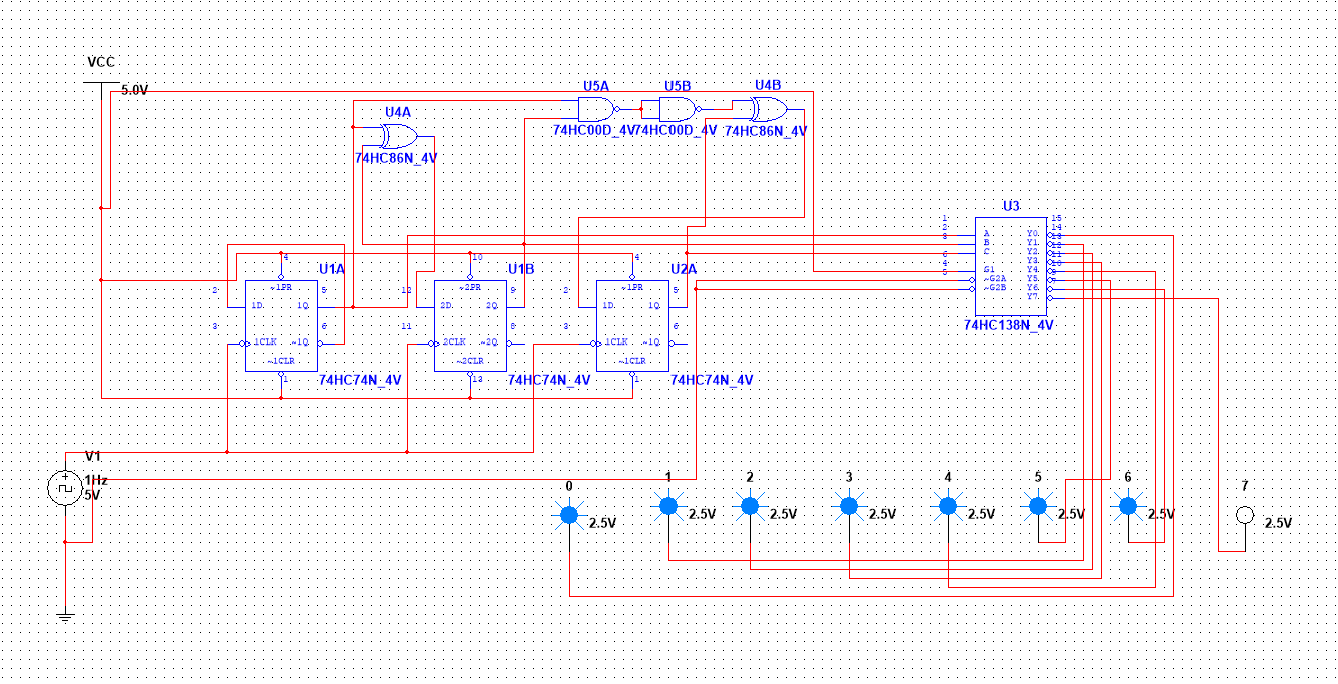
\includegraphics[width=0.8\textwidth]{../Ex1/img/Lab5_Ex1.png} % 确保文件名和路径正确
  \caption{广告流水灯逻辑电路图}\label{fig:circuit_diagram}
\end{figure}
\section{实验仪器}

\section{实验记录}
根据电路图搭接电路,将面包板上的连续脉冲信号接入CP端,将信号频率设置为\SI{1}{\hertz}。
将译码器的八个输出端接入面包板上的LED灯,进行动态验证。
之后,把CP信号的频率改为\SI{1000}{\hertz},依次把CP端、$\mathrm{Q_2}$、$\mathrm{Q_1}$、$\mathrm{Q_0}$和LED灯的输出端接入示波器,观察并记录波形。
示波器波形实物图如图\ref{fig:experiment_setup5}和图\ref{fig:experiment_setup7}所示。
汇总后的波形图如图\ref{fig:wavesummary}所示。
\begin{figure}[htbp]
    \centering
    % \renewcommand{\thefigure}{图\arabic{figure}}  % 修改图片编号格式为"图X"
    \begin{minipage}[t]{0.48\textwidth}
        \centering
        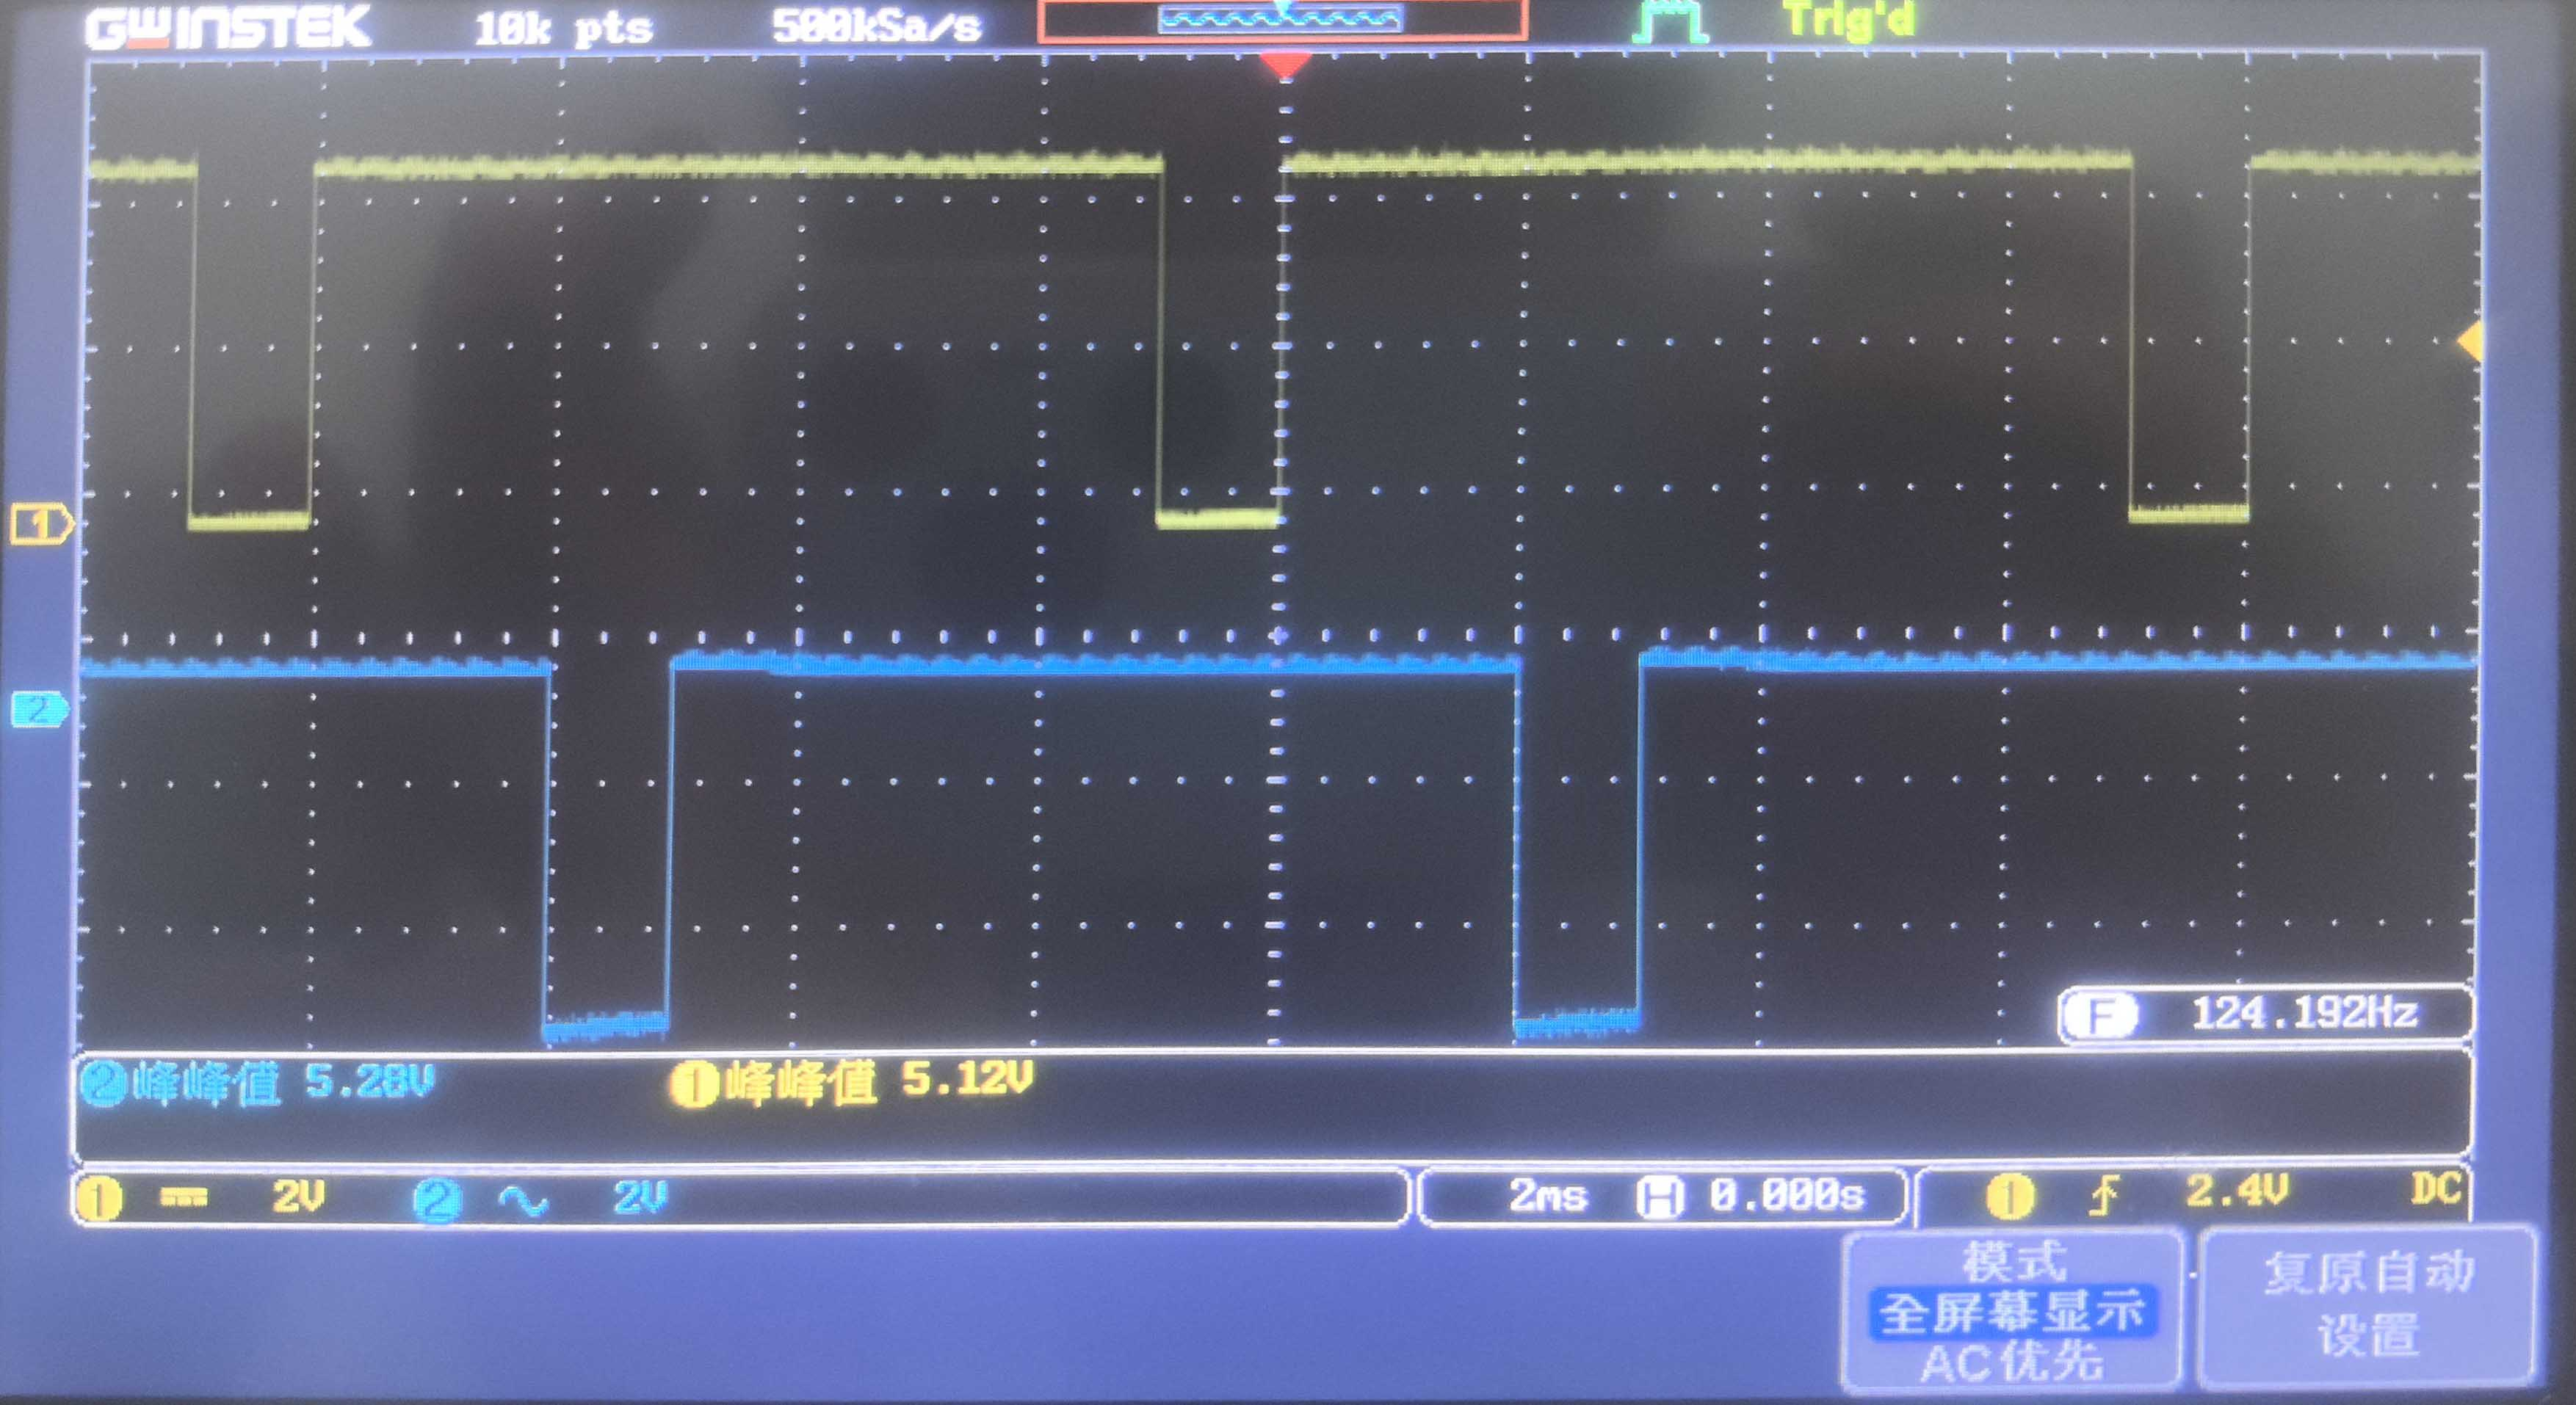
\includegraphics[width=\textwidth]{../Ex1/img/05.jpg}
        \caption{示波器显示波形实物图(0号灯和5号灯)}
        \label{fig:experiment_setup5}
    \end{minipage}
    \hfill
    \begin{minipage}[t]{0.48\textwidth}
        \centering
        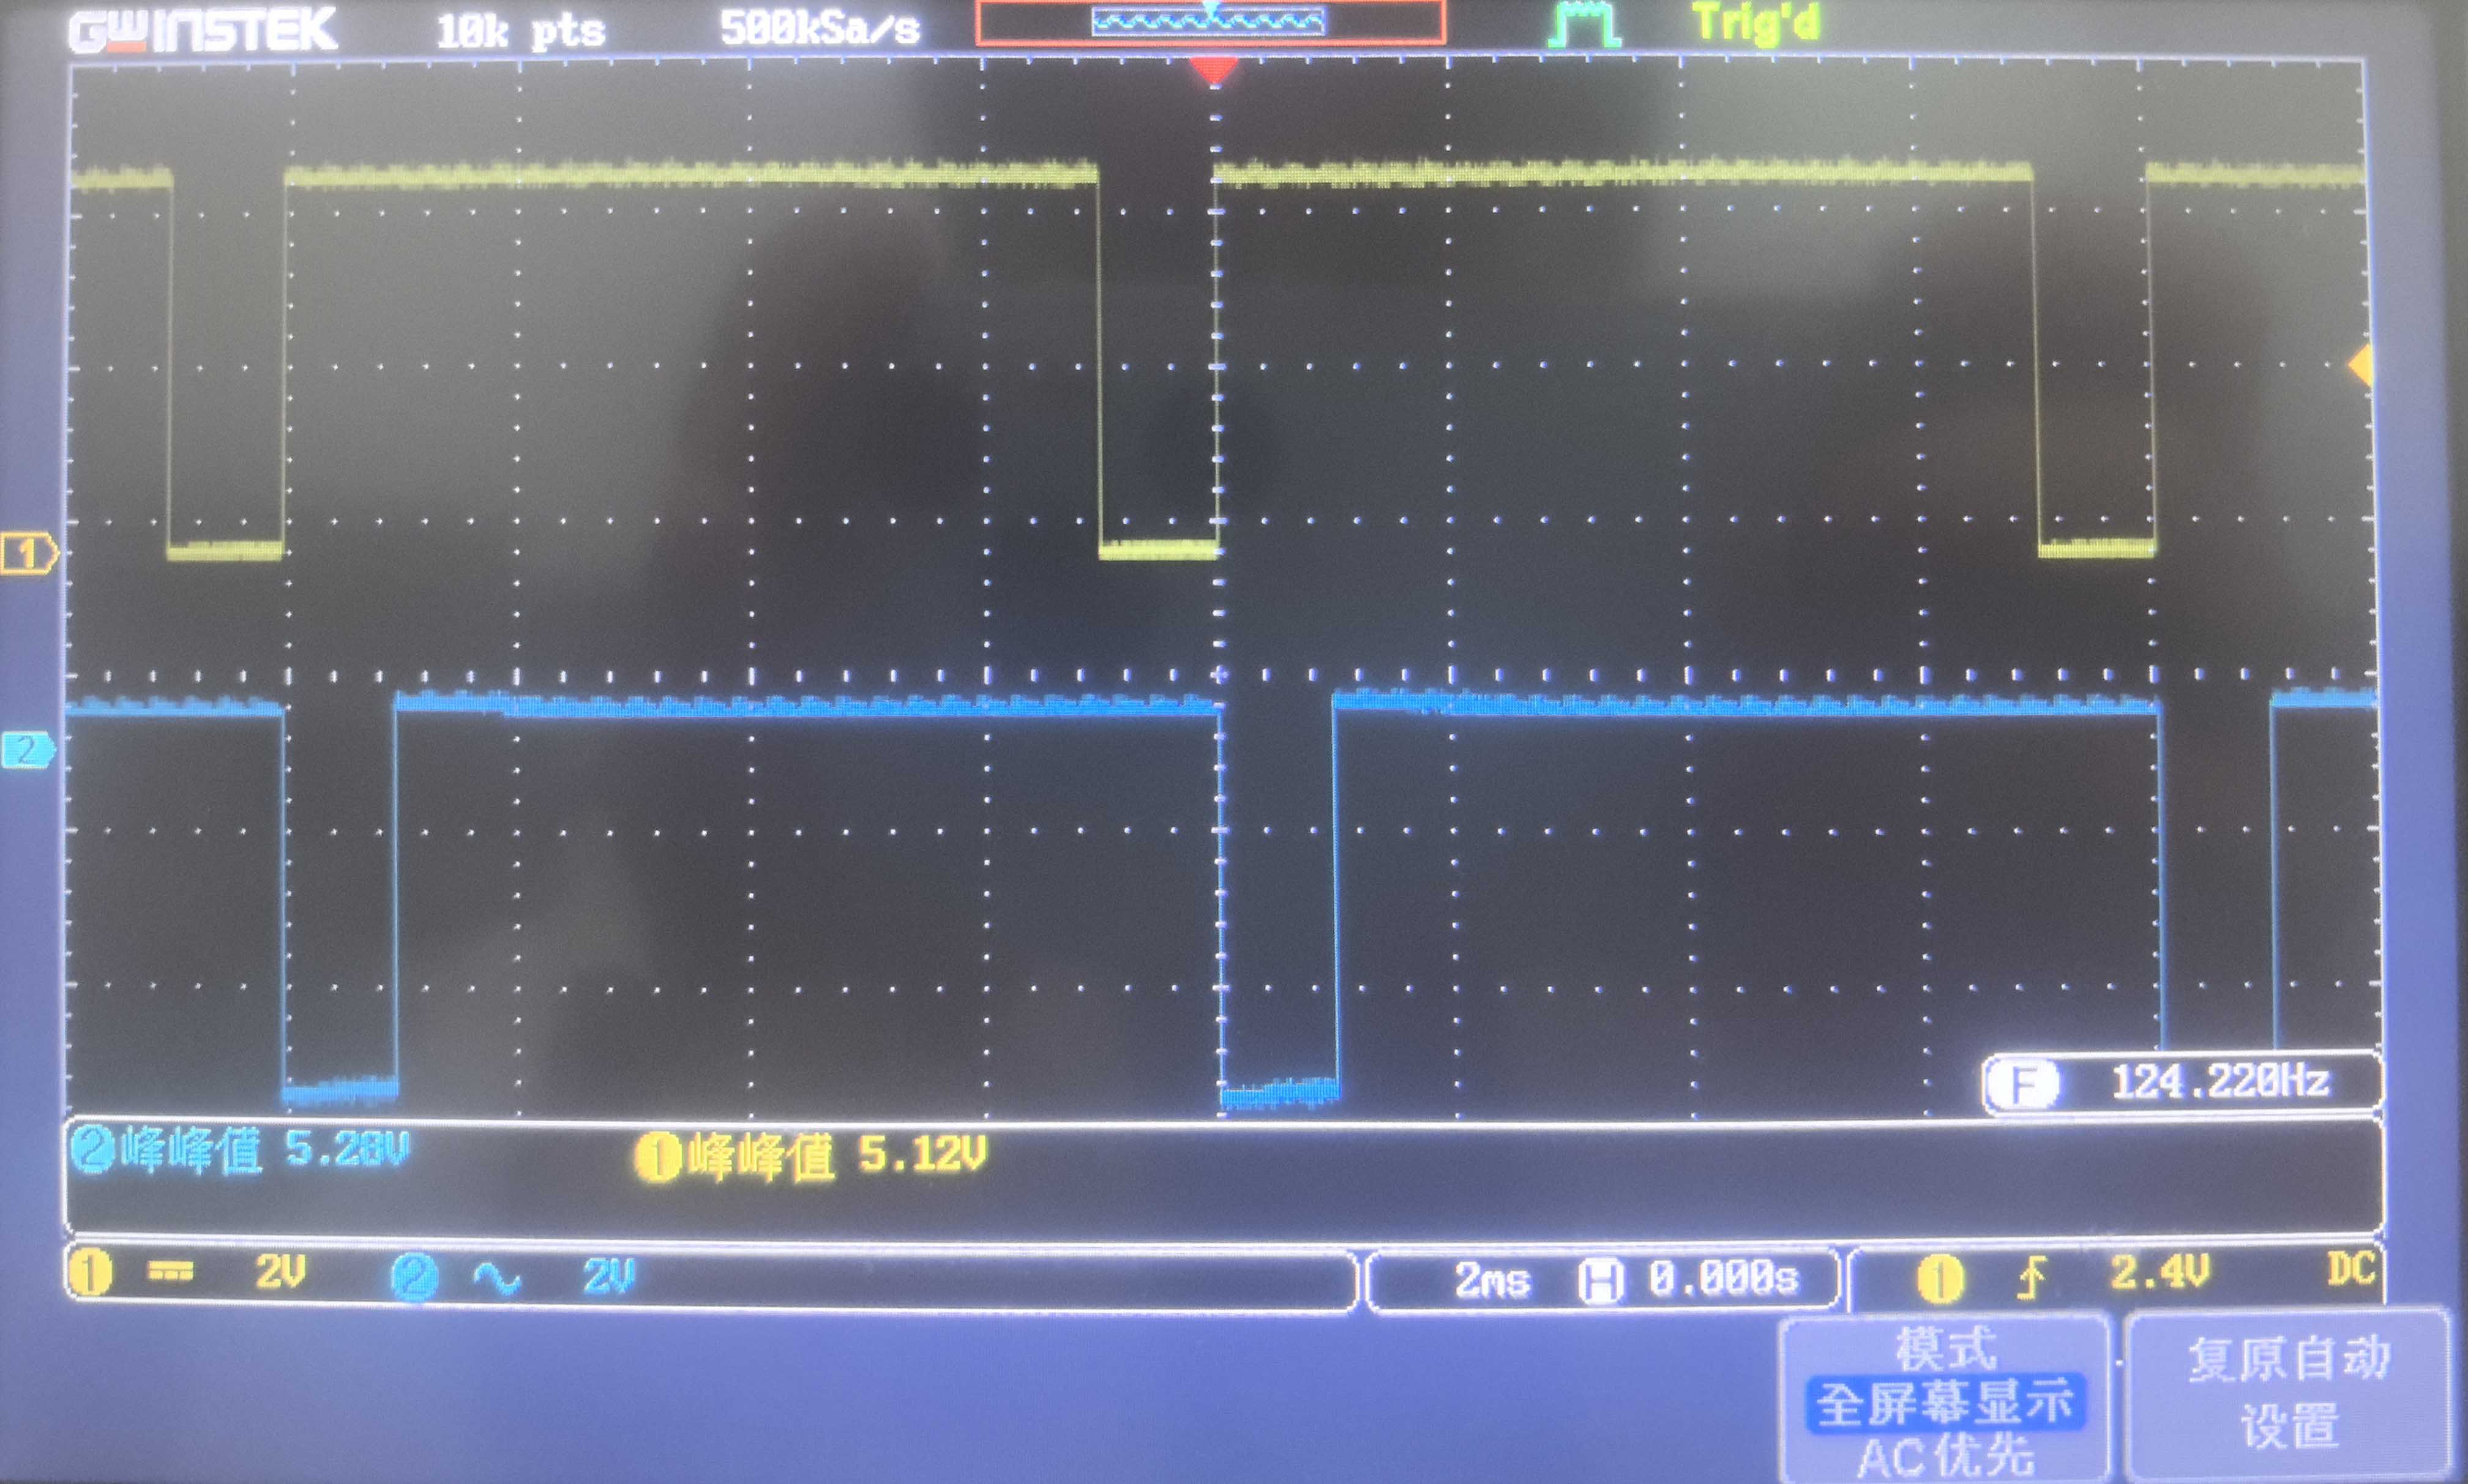
\includegraphics[width=\textwidth]{../Ex1/img/07.jpg}
        \caption{示波器显示波形实物图(0号灯和7号灯)}
        \label{fig:experiment_setup7}
    \end{minipage}
\end{figure}
\begin{figure}[htbp]
    \centering
    
\includegraphics[width=0.8\textwidth]{../Ex1/img/boxi.png}
    \caption{汇总后的波形图}
    \label{fig:wavesummary}
\end{figure}
\section{实验分析}
符不符合预期。

\section{实验小结}
瞎写点东西。
\end{document}